\documentclass[12pt]{report}
\usepackage[T1]{fontenc}
\usepackage[utf8]{inputenc}
\usepackage[italian]{babel}
\usepackage{amsmath}
\usepackage{amssymb}
\usepackage{graphicx}
\usepackage{listings}
\usepackage{xcolor}
\usepackage{titling}
\usepackage{listings}
\usepackage[a4paper,top=2cm, bottom=4cm, left=2cm,right=2cm]{geometry}
\usepackage[bottom]{footmisc}

\definecolor{codegreen}{rgb}{0,0.6,0}
\definecolor{codegray}{rgb}{0.5,0.5,0.5}
\definecolor{codepurple}{rgb}{0.58,0,0.82}
\definecolor{backcolour}{rgb}{0.95,0.95,0.92}

\lstdefinestyle{mystyle}{
	backgroundcolor=\color{backcolour},   
	commentstyle=\color{codegreen},
	keywordstyle=\color{magenta},
	numberstyle=\tiny\color{codegray},
	stringstyle=\color{codepurple},
	basicstyle=\ttfamily\footnotesize,
	breakatwhitespace=false,         
	breaklines=true,                 
	captionpos=b,                    
	keepspaces=true,                 
	numbers=left,                    
	numbersep=5pt,                  
	showspaces=false,                
	showstringspaces=false,
	showtabs=false,                  
	tabsize=2
}

\lstset{style=mystyle}

\begin{document}
	\author{Luca Fumagalli 939398\\ Lorenzo D'Alessandro 939416}
	\title{Relazione progetto \textit{Gestione dell’informazione geospaziale}\\Testo 1 }
	\date{\vspace{-5ex}}
	\maketitle
\chapter*{Struttura database}
Il nostro database è composto da sei tabelle:
\begin{itemize}
	\item \textbf{tragitto}: questa tabella contiene i punti originali acquisiti tramite GPS.
	\item \textbf{tragitto\_filtered}: tabella contenente i punti filtrati per tempo o distanza.
	\item \textbf{strade\_open\_street\_map}: tabella contenente i valori delle linestring rappresentanti le strade esportate da \textit{OpenStreetMap}.%
	\footnote{https://www.openstreetmap.org/}
	\item \textbf{matched\_point}: tabella contente i nuovi punti del tragitto dopo l'esecuzione dell'algoritmo di \textit{map matching}.
	\item \textbf{speed}: in questa tabella sono presenti le velocità tra coppie di punti del tragitto originale.
	\item \textbf{speed\_mm}: tabella contenente le stesse informazioni della tabella \textit{speed} ma calcolate sulla tabella \textit{matched\_point}.
\end{itemize}




\chapter*{Rilevamento traiettoria}
Per rilevare la traiettoria usta all'interno del progetto abbiamo utilizzato l'applicazione Android \textit{Geo Tracker - GPS tracker}%
\footnote{https://play.google.com/store/apps/details?id=com.ilyabogdanovich.geotracker\&hl=it}.
\begin{figure}
	\centering
	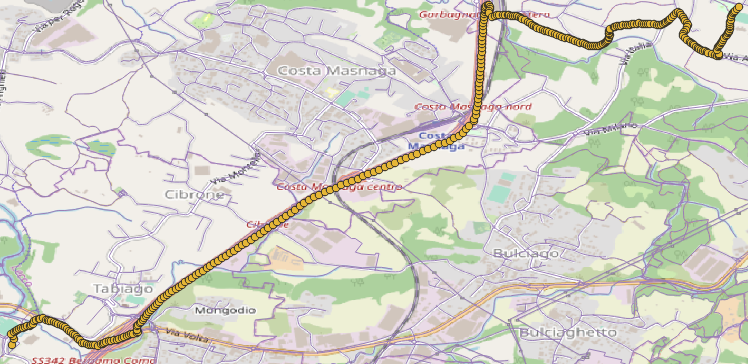
\includegraphics[scale = 0.43]{figures/punto1}
	\caption{Immagine presa da QGIS della mappa e della traiettoria}\label{punto1}
\end{figure}
Le geometrie delle strade sono state esportate dal sito di \textit{OpenStreetMap}.

Il risultato dell'acquisizione della traiettoria e la sovrapposizione alla mappa è visibile in figura \ref{punto1}.

\chapter*{Map Matching}
Per eseguire l'algoritmo di \textit{map matching} abbiamo effettuato diverse operazioni:
\begin{itemize}
	\item Come prima operazione abbiamo dovuto prendere tutti i dati del tragitto dal database ed inserirli in una lista, ogni punto è rappresentato da una tupla i cui elementi sono le colonne della tabella \textit{tragitto} del database. \lstinputlisting[language=SQL]{code/query1.sql}
	\item Per ogni punto del tragitto cerchiamo la \textit{linestring} corrispondente alla strada più vicina. Per ogni punto creiamo una tupla formata dall'\textit{id} del punto e l'\textit{id} della strada più vicina che viene inserita nella lista \textit{point\_closest\_line\_list} \lstinputlisting[language=SQL]{code/query.sql}\lstinputlisting[language=Python]{code/python.py}
	\item Viene effettuato il \textit{fix} sui punti che si trovano isolati su una strada. \lstinputlisting[language=Python]{code/fix.py}
	\item Viene proiettato il punto sulla strada più vicina e viene inserito nel database nella tabella \textit{matched\_point}.
	\lstinputlisting[language=SQL]{code/match.sql}\lstinputlisting[language=Python]{code/matched.py}
\end{itemize}
Il risultato visivo dell'esecuzione dell'algoritmo di map matching è rappresentato in figura \ref{mapmatching}.
\begin{figure}
	\centering
	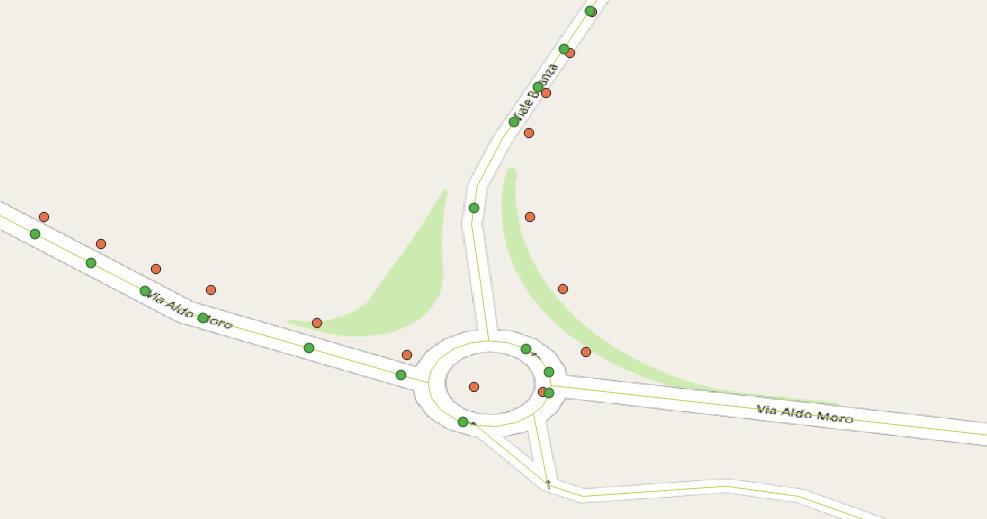
\includegraphics[scale = 0.43]{figures/mm}
	\caption{I punti arancioni sono i punti originali, quelli verdi i punti prodotti dal map matching.}\label{mapmatching}
\end{figure}
	
\chapter*{Velocità}
\begin{itemize}
	\item Come avviene per l'esecuzione dell'algoritmo di \textit{map matching}, creiamo una lista di tuple formate da \textit{id} del punto ed \textit{istante di tempo} in cui è stato registrato.
	\item Calcoliamo la differenza tra gli istanti di tempo($\Delta$t) di coppie successive di punti.\lstinputlisting[language=Python]{code/dt.py}
	\item Calcoliamo la distanza($\Delta$s) tra coppie successive di punti tramite query sql. Questa operazione viene effettuata sia sui punti originali che sui punti dopo l'esecuzione del map matching.\lstinputlisting[language=SQL]{code/distance.sql}\lstinputlisting[language=SQL]{code/distancemm.sql}
	\item Creiamo una lista di tuple formata da \textit{id primo punto}, \textit{id secondo punto}, \textit{$\Delta$t}, \textit{$\Delta$s}.
	\item Calcoliamo la velocità per ogni coppia di punti utilizzando la lista appena creata. Durante il calcolo della velocità tra i due punti viene anche aggiornata la velocità media totale.\lstinputlisting[language=Python]{code/speed.py}
	\item Vengono create due tabelle nel database, \textit{speed} e \textit{speed\_mm} relative alle velocità calcolate.
\end{itemize}
\chapter*{Riduzione numero punti}
Per ridurre il numero di punti abbiamo due possibilità: filtrare i dati in base all'istante di tempo in cui sono stati acquisiti oppure in base alla distanza tra due punti.
\begin{itemize}
	\item \textbf{Istante di tempo:} data una funzione che prende un parametro \textit{t} come input, viene creata una lista \textit{points\_filtered} contenente solo i punti la cui distanza temporale è $ \ge t $ .\lstinputlisting[language=Python]{code/filter.py}
	
	Il risultato dell'applicazione del filtro è visibile in figura \ref{filter}.
	\item \textbf{Distanza tra punti:} data una funzione che prendere un parametro \textit{t} come input, viene creata una lista \textit{points\_filtered} contente solo i punti la cui distanza è $ \ge t$ metri. \lstinputlisting[language=Python]{code/filter2.py}
	
\end{itemize}
	\begin{figure}
	\centering
	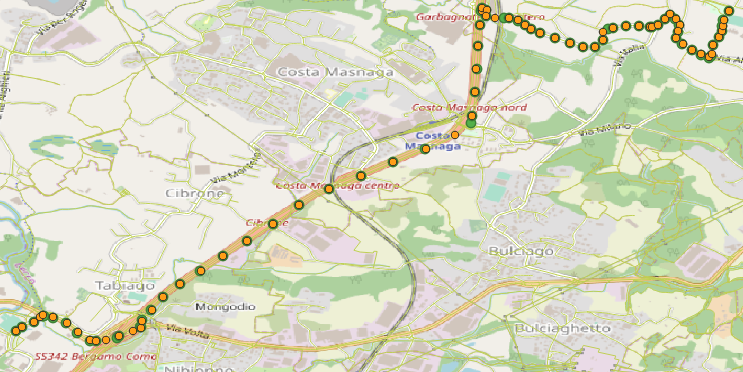
\includegraphics[scale = 0.43]{figures/tragitto_filtered}
	\caption{Tragitto originale e risultato del map matching dopo l'utilizzo del filtro.}\label{filter}
\end{figure}
	
	
	
\end{document}